\subsection{UC S- Sincronizzare} \label{sec:UCS}
    \begin{figure}[h]
        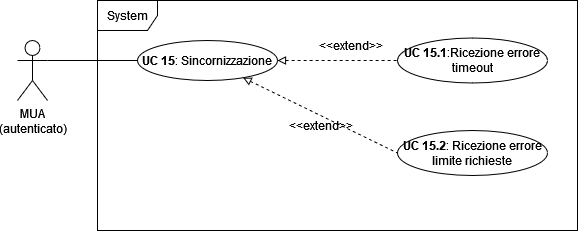
\includegraphics[width=0.85\textwidth]{sections/uc_imgs/UCS.png}
        \centering
        \caption{Diagramma UC S }
    \end{figure}
    \begin{itemize}
        \item \textbf{Attore principale}: MUA;
        \item \textbf{Descrizione}: il MUA richiede la sincronizzazione con gli oggetti del sistema;
        \item \textbf{Precondizioni}: l’account che il MUA gestisce è registrato nel sistema, e ha un connessione aperta con il sistema ed è autenticato;
        \item \textbf{Postcondizioni}: il MUA è sincronizzato con i dati presenti nel sistema;
        \item \textbf{Scenario principale}:
            \begin{enumerate}
                \item il MUA invia i dettagli necessari ad indentificare gli oggetti da Sincronizzare;
                \item il sistema invia al MUA gli aggiornamenti;
            \end{enumerate}
        \item \textbf{Inclusioni}: nessuna;
        \item \textbf{Generalizzazioni}: nessuna;
            % tho la sincronizzazione è fatta per oggetto con jmap
            %\begin{itemize}
            %    \item il MUA sincronizza contatti (\hyperref[sec:UC12]{UC 12});
            %    \item il MUA sincronizza eventi nel calendario (\hyperref[sec:UC13]{UC 13});
            %    \item il MUA sincronizza cartelle (\hyperref[sec:UC14]{UC 14});
            %\end{itemize}
        \item \textbf{Estensioni}: 
        \begin{itemize}
            \item il sistema ritorna un errore al MUA per timeout (\hyperref[sec:UC11.2]{UC 11.2}).
            \item il sistema ritorna un errore al MUA per limite richieste (\hyperref[sec:UC11.2]{UC 11.2}).

        \end{itemize}
    \end{itemize}


    \subsubsection{UC S.1 - Ricezione errore timeout} \label{sec:UCS.1}
    \begin{itemize}
        \item \textbf{Attore principale}: MUA;
        \item \textbf{Descrizione}: il sistema non riesce a sincronizzarsi perché il tempo necessario per completare l'operazione supera il limite di timeout;
        \item \textbf{Precondizioni}: il MUA sta usando la funzionalità sincronizzazione;
        \item \textbf{Postcondizioni}: il sistema non invia al MUA gli aggiornamenti, il MUA è stato notificato dell'errore;
        \item \textbf{Scenario principale}:
            \begin{enumerate}
                \item l'operazione richiesta supera il tempo massimo previsto dal sistema;
                \item il sistema non invia gli aggiornamenti e notifica il MUA dell'errore;
            \end{enumerate}
        \item \textbf{Inclusioni}: nessuna;
        \item \textbf{Generalizzazioni}: nessuna;
        \item \textbf{Estensioni}: nessuna.
    \end{itemize}

    \subsubsection{UC S.2 - Ricezione errore limite richieste} \label{sec:UCS.2}
    \begin{itemize}
        \item \textbf{Attore principale}: MUA;
        \item \textbf{Descrizione}: il sistema non riesce a sincronizzarsi perché il MUA supera la quantità massima di richieste al server;
        \item \textbf{Precondizioni}: il MUA sta usando la funzionalità sincronizzazione;
        \item \textbf{Postcondizioni}: il sistema non invia al MUA gli aggiornamenti, il MUA è stato notificato dell'errore;
        \item \textbf{Scenario principale}:
            \begin{enumerate}
                \item il MUA supera la quantità massima di richieste da mandare al sistema;
                \item il sistema non invia gli aggiornamenti e notifica il MUA dell'errore;
            \end{enumerate}
        \item \textbf{Inclusioni}: nessuna;
        \item \textbf{Generalizzazioni}: nessuna;
        \item \textbf{Estensioni}: nessuna.
    \end{itemize}

